%% Manuscript for the effect of designed conversational architecture on the perception of agents
%%
%% The first command in your LaTeX source must be the \documentclass command.
\documentclass[sigconf,screen,review, anonymous]{acmart}

\usepackage[linewidth=1pt]{mdframed}
\usepackage{lipsum}
\usepackage{multirow}
\usepackage{graphicx}
\usepackage{booktabs}

\newcommand{\cmt}[1]{}%{\ignorespaces}


%% NOTE that a single column version may be required for 
%% submission and peer review. This can be done by changing
%% the \doucmentclass[...]{acmart} in this template to 
%% \documentclass[manuscript,screen]{acmart}
%% 
%% To ensure 100% compatibility, please check the white list of
%% approved LaTeX packages to be used with the Master Article Template at
%% https://www.acm.org/publications/taps/whitelist-of-latex-packages 
%% before creating your document. The white list page provides 
%% information on how to submit additional LaTeX packages for 
%% review and adoption.
%% Fonts used in the template cannot be substituted; margin 
%% adjustments are not allowed.
%%
%%
%% \BibTeX command to typeset BibTeX logo in the docs
\AtBeginDocument{%
  \providecommand\BibTeX{{%
    \normalfont B\kern-0.5em{\scshape i\kern-0.25em b}\kern-0.8em\TeX}}}

%% Rights management information.  This information is sent to you
%% when you complete the rights form.  These commands have SAMPLE
%% values in them; it is your responsibility as an author to replace
%% the commands and values with those provided to you when you
%% complete the rights form.
\setcopyright{acmcopyright}
\copyrightyear{2023}
\acmYear{2023}
\acmDOI{XXXXXXX.XXXXXXX}

%% These commands are for a PROCEEDINGS abstract or paper.
\acmConference[Conference acronym 'XX]{Make sure to enter the correct
  conference title from your rights confirmation email}{June 03--05,
  2018}{Woodstock, NY}
%
%  Uncomment \acmBooktitle if th title of the proceedings is different
%  from ``Proceedings of ...''!
%
%\acmBooktitle{Woodstock '18: ACM Symposium on Neural Gaze Detection,
%  June 03--05, 2018, Woodstock, NY} 
\acmPrice{15.00}
\acmISBN{978-1-4503-XXXX-X/18/06}

%%
%% Submission ID.
%% Use this when submitting an article to a sponsored event. You'll
%% receive a unique submission ID from the organizers
%% of the event, and this ID should be used as the parameter to this command.
%%\acmSubmissionID{123-A56-BU3}

%%
%% end of the preamble, start of the body of the document source.
\begin{document}
%TC:ignore

%%
%% The "title" command has an optional parameter,
%% allowing the author to define a "short title" to be used in page headers.
% \title[short title]{How to Make Pinocchio a Real Boy? Designing conversational architecture elements to achieve desirable anthropomorphized perceptions}
\title[Bot's Guide to Being Human]{Bot's Guide to Being Human: Investigating the Effect of Conversation Architecture Elements on the Anthropomorphized Perceptions of Conversational Agents}
% Blurring the line between human and bots


%%
%% The "author" command and its associated commands are used to define
%% the authors and their affiliations.
%% Of note is the shared affiliation of the first two authors, and the
%% "authornote" and "authornotemark" commands
%% used to denote shared contribution to the research.
\author{Christina Wei}
\email{christina.wei@mail.utoronto.ca}
\affiliation{%
  \institution{University of Toronto}
  \city{Toronto}
  \country{Canada}
}

\author{Young-Ho Kim}
\email{ygho.kim@navercorp.com}
\affiliation{%
  \institution{Naver Corporation}
  \city{Seoul}
  \country{Korea}
}

\author{Anastasia Kuzminykh}
\email{anastasia.kuzminykh@utoronto.ca}
\affiliation{%
  \institution{University of Toronto}
  \city{Toronto}
  \country{Canada}
}

%%
%% By default, the full list of authors will be used in the page
%% headers. Often, this list is too long, and will overlap
%% other information printed in the page headers. This command allows
%% the author to define a more concise list
%% of authors' names for this purpose.
\renewcommand{\shortauthors}{Wei, Kim, and Kuzminykh}

%%
%% The abstract is a short summary of the work to be presented in the
%% article.
\begin{abstract}
  TBD
\end{abstract}

%%
%% The code below is generated by the tool at http://dl.acm.org/ccs.cfm.
%% Please copy and paste the code instead of the example below.
%%
\begin{CCSXML}
<ccs2012>
 <concept>
  <concept_id>10010520.10010553.10010562</concept_id>
  <concept_desc>Computer systems organization~Embedded systems</concept_desc>
  <concept_significance>500</concept_significance>
 </concept>
 <concept>
  <concept_id>10010520.10010575.10010755</concept_id>
  <concept_desc>Computer systems organization~Redundancy</concept_desc>
  <concept_significance>300</concept_significance>
 </concept>
 <concept>
  <concept_id>10010520.10010553.10010554</concept_id>
  <concept_desc>Computer systems organization~Robotics</concept_desc>
  <concept_significance>100</concept_significance>
 </concept>
 <concept>
  <concept_id>10003033.10003083.10003095</concept_id>
  <concept_desc>Networks~Network reliability</concept_desc>
  <concept_significance>100</concept_significance>
 </concept>
</ccs2012>
\end{CCSXML}

\ccsdesc[500]{Computer systems organization~Embedded systems}
\ccsdesc[300]{Computer systems organization~Redundancy}
\ccsdesc{Computer systems organization~Robotics}
\ccsdesc[100]{Networks~Network reliability}

%%
%% Keywords. The author(s) should pick words that accurately describe
%% the work being presented. Separate the keywords with commas.
\keywords{conversational agents, user perception, conversational architecture, social cues}

%%\received{20 February 2007}
%%\received[revised]{12 March 2009}
%%\received[accepted]{5 June 2009}

%%
%% This command processes the author and affiliation and title
%% information and builds the first part of the formatted document.
\maketitle
%TC:endignore

\section{Introduction}

Conversational agents (CAs) are software-based systems, either voice of text-based, designed to interact with humans using natural language. Adoption for CAs such as Alexa (Amazon) or Siri (Apple) are rapidly growing in the market, with half of US internet users own one or more smart speaker devices \cite{2022comscore}. These conversational agents are designed to be ubiquitous, easily accessible through smartphones, tablets, laptops and smart devices. Because these agents leverage natural language for interaction, they solicit social responses from users, encouraging users to attribute lifelike qualities, a.k.a. anthropomorphized perceptions to CAs \cite{eyssel2012if}.

Anthropomorphism is defined as the attribution of traits that we typically associate with being distinctly human to nonhuman entities \cite{waytz2010sees}. For example, users tend to personify conversational agents like Amazon Alexa by using person pronouns instead of object pronouns in online reviews \cite{purington2017alexa}.  Research shows that anthropomorphic design is beneficial to establishing and maintaining trust between users and conversational agents \cite{seeger2021chatbots}. Also, speakers tend to align their lexical choices with conversational agents, similar to human-human conversations \cite{cowan2015does}. Anthropomorphism has been shown to ease user interactions, e.g. making agents more approachable, engaging, and trustworthy when they exhibit human characteristics \cite{qiu2009evaluating}. These processes are of particular interest for human-agent communication because they form the basis for user expectations and predispositions regarding agents' behavior, reliability of the information, etc. \cite{kuzminykh2020genie}.

One of the key factors for anthropomorphized perception is how conversational agents convey information through verbal or non-verbal cues. Studies have found that conversational agents are perceived as more socially present and emotionally intelligent if they use sentiment-adaptive response based on user's utterances, resulting in higher user satisfaction \cite{diederich2019emulating}\cite{yang2017perceived}. Also, CAs that mimic user behaviour through lexical alignment reduce users' cognitive workload, resulting in higher engagement with the interaction \cite{spillner2021talk}. Non-verbal cues such as expressive prosody contribute to higher perceived intimacy with the user, as well as higher perceived enjoyment and ease of use \cite{kim2020can}. However, conversational architecture design may lead to negative consequences, such as an agent with an extroverted personality may be seen as less trustworthy, as users are irritated by the system's overly familiar attitude \cite{andrews2012system}.

Even though there are existing research efforts investigating the effect of various conversational architecture elements on the anthropomorphized perception of agents, there is no clear view on the overall landscape on the state of research to understand what has been studied and what needs more efforts. Some reasons for this gap could be due to the lack of consistency in perception measures such as humanness or empathy. There are various questionnaires used in the studies (e.g. Godspeed Questionnaire) but their definitions for perceptions may be different. Also, there are various confounding factors like prior experience and domain of usage that makes it hard to generalize design principles for anthropomorphized perception of agents.

This paper attempts to address this gap in knowledge by investigating the following research questions: (RQ1) How does the specifics of conversational architecture design affect the anthropomorphized perception of CAs? and (RQ2) How does the specifics of conversational architecture design affect the perception of interaction with CAs? Through a comprehensive review of the existing literature, this paper presents the synthesis of a design framework developed based on X number of paper published between 2010 and 2022. The framework associated four categories of perception - interaction, ability of the agent, human attributes of the agent, and social connections with the user, with four categories of conversational architecture elements - verbal (content, style), visual (CMC), auditory (voice qualities, vocalizations), and chronemics adapted from Feine et al \cite{feine2019taxonomy}.

<One paragraph summarizing results>

<One paragraph outlining contributions to the HCI community>
* Synthesize existing framework into design framework \newline
* Point out gaps in research \newline

In the remainder of the paper, we first review the existing literature on design frameworks for conversational agents and measures of anthropomorphized perceptions. We then describe our literature review and data analysis process, following by describing the design framework synthesized based on findings of the collected literature corpus. Finally, we discuss the critical gaps in research identified through our analysis, and propose key opportunities for future research.


Design the conversational agents


%\section{Literature Review}

%\cite{finch2020towards} Towards unified dialogue system evaluation: A comprehensive analysis of current evaluation protocols

%Synthesis on conversational architecture

%Synthesis on measures

%Connections between conversational architecture elements and measures


\section{Methods}

This section describes the research methodologies for the search procedure, selection criteria and data analysis process.

\subsection{Search Procedure}

Following PRISMA guidelines \cite{prisma}, we reviewed and selected literature relevant to the relationships between the specifics of conversation architecture elements and anthropomorphized perceptions of CAs. Searches were carried out in the ACM Digital Library between January 1 and January 15, 2023. During initial analysis, it didn't seem like there were common terms used to refer to either conversation architecture elements, or anthropomorphized perceptions. As such, search terms were kept general to literature related to conversational agents. Based on search terms used in previously published literature reviews \cite{clark2019state}\cite{rapp2021human} , the following keywords have been identified to search for publications related to conversational user interfaces:
\newline

\begin{mdframed}
"conversational agent" OR "natural language interface" OR "IPA" OR "intelligent personal assistant" OR "chatbot" OR "speech interface" OR "voice assistant" OR "intelligent agent" OR "human-chatbot communication" OR "virtual agent" OR "dialog* system" OR "voice user interface" OR "human computer dialog*"
\end{mdframed}

\subsection{Selection Criteria}
The initial query retrieved 2901 unique publications. The following selection criteria are applied to identify literature related to the effect of conversational architecture on perception of agents:
\begin{itemize}
  \item Peer-reviewed publications written in English
  \item Voice-based or text-based conversational agents
  \item Experiment study on the impact of conversation architecture elements on the anthropomorphized perceptions of agents
  \item Impact of conversation architecture elements can be separated from other effects (e.g. embodiment)

\end{itemize}

We screened the titles and abstracts of the papers based on the selection criteria below which resulted in 221 papers. Reviewing the full articles of these publication resulted in 49 papers for analysis. An additional search for related literature was also performed to find new publications, adding 8 more papers to the corpus. We identified 57 relevant articles that met our selection criteria (see Figure \ref{fig:prisma}).

\begin{figure}[h]
  \centering
  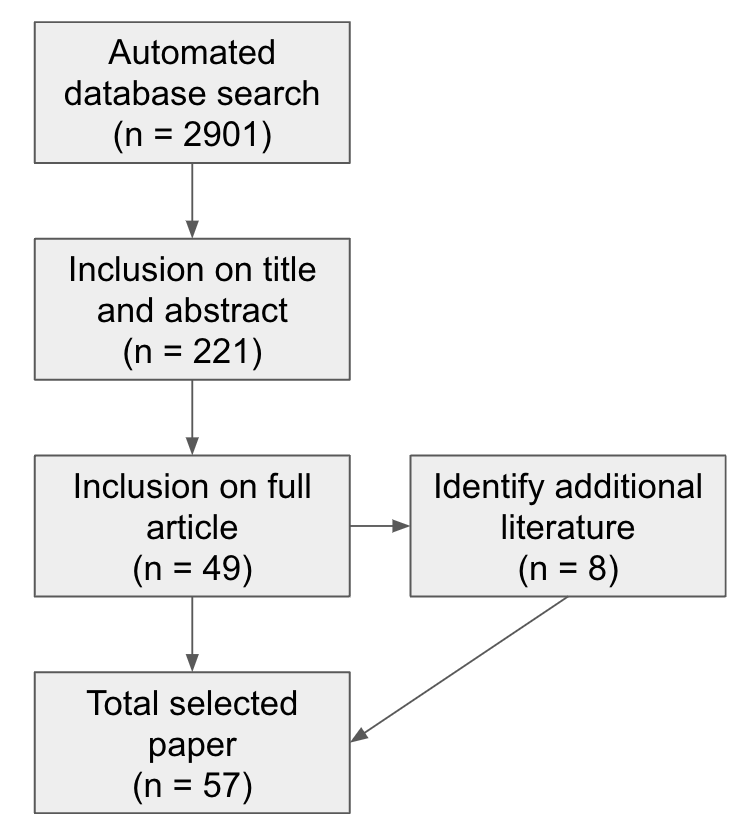
\includegraphics[width=0.6\columnwidth]{fig-prisma.png}
  \caption{Literature search using PRISMA guidelines}
  \label{fig:prisma}
\end{figure}

\subsubsection*{Literature Corpus Characteristics}

The papers reviewed (n=57) were published between May 2011 and November 2022. More than 75\% of the papers were published in or after 2019, with a slight trend upwards over the years (see Figure \ref{fig:paper}). The vast majority of the papers in our corpus were published in conference proceedings (n=50), with the remainder papers published in journals. Out of the papers published in conferences, the top conferences were The ACM Conference on Human Factors in Computing Systems (n=16), Conversational User Interfaces (n=7), Human-Agent Interaction (n=4), and Intelligent Virtual Agents (n=4). Out of the papers published in journals, some venues include the International Journal of Human-Computer Interaction (n=2) and Interacting with Computers (n=1).

On the modality characteristics of the conversational agents in the corpus, there is a roughly even split between the modalities, with slightly more papers (n=30) studying voice-based CAs, and the rest (n=27) studying text-based CAs.

\begin{figure*}[h]
  \centering
  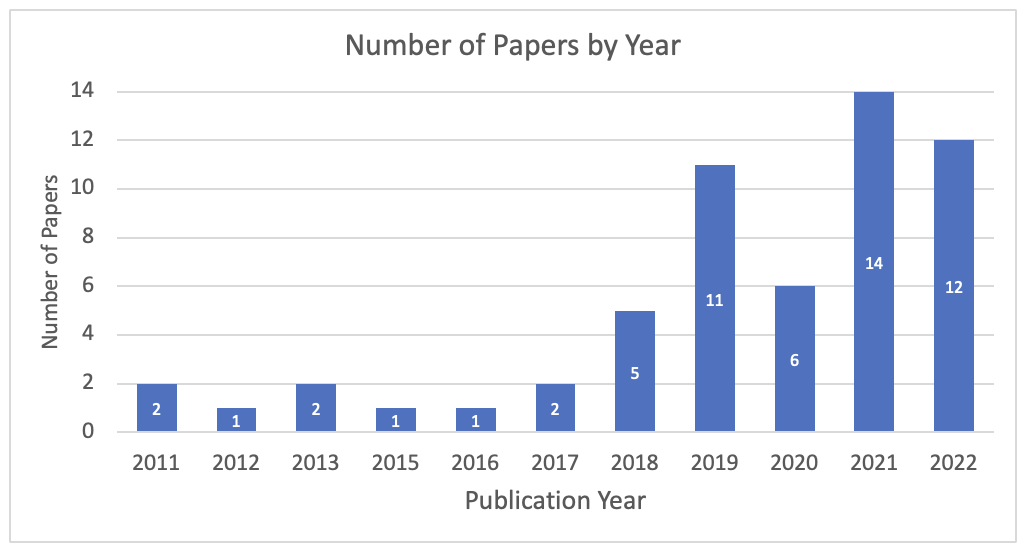
\includegraphics[width=\textwidth]{fig-paper.png}
  \caption{Stacked barchart of number of papers by year and venue}
  \label{fig:paper}
\end{figure*}

\subsection{Data Analysis}

\subsubsection*{Anthropomorphized Perceptions}
The exact quotes of anthropomorphized perception measurements were extracted from each paper. Inductive thematic analysis was used to group these verbatim quotes into codes based on their meanings. For example, the code likeability of the agent contains the questionnaire item "this voice agent was likeable" used by \cite{cuadra2021my}\cmt{[67]}, Godspeed questionnaire \cite{bartneck2009measurement}\cmt{godspeed}'s set of questions on likeability used by \cite{linnemann2018can}\cmt{[15]}, and Subjective Assessment of Speech System Interface (SASSI) questionnaire \cite{hone2000towards}\cmt{sassi}'s set of questions on likeability used by  \cite{chan2021kinvoices}\cmt{[74]}\cite{choi2020nobody}\cmt{[54]}. This step resulted in 83 unique codes. The codes are then organized based similarity of the meanings, resulting in 11 basic themes. For example, the basic theme of \textit{personality traits} of the agent contains measurements such as likeability, friendliness, and warmth. Lastly, the 11 basic themes are categorized into 4 organizing themes: \textit{perception of interaction with agent, perception of agent's ability, perception of social connection with agent, and perception of agent's humanness} (Table \ref{tab:perceptions}).

\subsubsection*{Conversation Architecture Elements}
The conversation architecture elements used in the study were extracted from each paper. Some of the papers were applying multiple elements to the CA design, such as the the anthropomorphic design used in this study \cite{seeger2021chatbots}\cmt{[35]}. In the case where multiple elements were used, the codes broke down the conversation architecture into its core components. For example, the anthropomorphic design used in Seeger et al's study \cite{seeger2021chatbots}\cmt{[35]} was broken down to the elements of emotional expressions, is-typing indicator, emoticons, and response delay to capture as codes. 58 unique codes were created as part of this process, capturing elements like sentiment-adaptive responses \cite{diederich2019emulating}\cmt{[25]}, lexical alignment \cite{spillner2021talk}\cmt{[18]}, and typos \cite{westerman2019believe}\cmt{[9]}. Codes were then organized based on similarity of the elements. For example, the basic theme of \textit{disfluency} contains elements of fillers \cite{jeong2019exploring}\cmt{[10]}\cite{wester2015artificial}\cmt{[14]}, interjections \cite{ceha2022expressive}\cmt{[77]}\cite{hu2021enhancing}\cmt{[56]}, and repetitions \cite{yang2021effect}\cmt{[72]}. Lastly, these basic themes are then categorized into organizing themes adapted from the social cues taxonomy structure by Feine et al \cite{feine2019taxonomy}. Based on this paper, the Verbal-Content category is mapped to our organizing theme of \textit{linguistic content}, and the Verbal-Style category is mapped to our organizing theme of \textit{linguistic style}.
Given our analysis focuses on the text and voice aspects of a conversational agent and does not analyze the embodiment aspects of design, the visual category is not applicable for our analysis. Also, we collapsed the auditory and invisible categories into the organizing theme of \textit{non-linguistic format} (Table \ref{tab:cues}).

\subsubsection*{Relationship Between Anthropomorphized Perceptions and Conversation Architecture Elements}
Based on the codes developed for anthropomorphized perceptions and conversation architecture elements above, we extracted the relationships between perceptions and architecture elements from each paper, noting whether the architecture element had an impact of on the perceptions. Out of the 57 papers, 264 connections between anthropomorphized perceptions and conversation architecture elements were found. To analyze specifically the relationships between the specifics of conversation architecture that affect the anthropomorphized perceptions of CAs, 69 connections that did not result in significant relationships were discarded, resulting in 195 relationships for analysis. For example, the specific connection between style matching and user satisfaction was discarded because Hoegen et al. \cite{hoegen2019end}\cmt{[31]} did not find a significant difference between the style matching agent and the non-style matching agent for overall interaction satisfaction. Out of the 195 relationships, 185 were relationships between individual architecture elements and perceptions. These single architecture element to perception relationships are visualized as a heatmap based on literature coverage within the literature review corpus, as seen in Figure \ref{fig:heatmap-impact}. Perceptions impacted by the composite of multiple architecture elements in an agent will be discussed in more details in the Composite Architecture Elements section.

\section{Findings}

TBD

\subsection{Anthropomorphized Perceptions}

\begin{table*}[]
\resizebox{\textwidth}{!}{%
\begin{tabular}{@{}lllc@{}}
\toprule
\textbf{Category} & \textbf{Theme}   & \textbf{Sample Codes}                                  & \textbf{No. Papers} \\ \midrule
\multirow{3}{*}{Perception of Interaction with Agent}    & Usability       & accuracy, ease of use, efficiency, helpfulness & 23 \\
 & Engagement         & enjoyment, annoyance, desirable, intention to use  & 28         \\
 & Satisfaction       & service satisfaction, quality of interaction       & 12         \\ \midrule
\multirow{3}{*}{Perception of Agent's Ability}              & Intelligence    & knowledgeable, intelligent, expertise                             & 11 \\
 & Competence         & competent, capable                                 & 4          \\
 & Trust              & credibility, trustworthy, truthfulness, confidence & 15         \\ \midrule
\multirow{3}{*}{Perception of Social Connection with Agent}  & Conversation Tone  & appropriate, expressive, empathetic, persuasive    & 13 \\
 & Social Presence & connectedness, familiarity, similarity, psychological distance    & 18        \\
 & Intimacy           & intimate, rapport, quality of relationship         & 7          \\ \midrule
\multirow{2}{*}{Perception of Agent's Humanness}            & Human-likeness  & human-like, natural, artificial, machine-like                     & 20 \\
 & Personality Traits & friendly, kind, warm, creepy, likeable, polite     & 27         \\ \bottomrule
\end{tabular}%
}
\caption{Perception measures}
\label{tab:perceptions}
\end{table*}

As shown in Table \ref{tab:perceptions}, there are four organizing themes defined for the anthropomorphized perceptions of conversational agents covering 11 basic themes of perception. The details of each theme are discussed below.

\textbf{Perception of interaction with a CA} evaluates the overall interaction quality users had with the conversational agent. The three basic themes for this perceptions are usability, engagement and satisfaction. \textit{Usability} measures the utilitarian aspects of the interaction, whether it was accurate, easy to use, efficient or helpful. Some commonly used methods to measure usability include the response accuracy portion of the SASSI questionnaire \cite{hone2000towards}\cmt{sassi}, or the NASA Task Load Index (NASA-TLX) \cite{hart1988development}\cmt{nasa} to measure cognitive workload. Questions such as "the system is easy to use" or "it is easy to understand the agent" are also measures of usability. \textit{Engagement} on the other hand measures users' emotional reactions, whether they have enjoyed the conversation with CA, or annoyed or frustrated with the interaction. Some commonly used methods to measure engagement include  the annoyance portion of the SASSI questionnaire \cite{hone2000towards}\cmt{sassi}, and the Use Engagement Scale (UES) \cite{o2018practical}\cmt{ues}. Questions such as "I enjoyed using the system" or "I felt frustrated with the agent" are also measures of engagement. Lastly, \textit{Satisfaction} measures users' overall satisfaction interacting with the agent. Questions such as "the overall assessment of conversing with the CA was satisfactory" are used to measure this perception.

\textbf{Perception of a CA's ability} evaluates the perceived capabilities of the agent. While there are some elements of system performance in this measure, the main aspect we are interested in is the perception differences for agents with identify system capabilities but with different architecture elements. Specifically, \textit{intelligence} measures the agent's expertise and knowledge, and it is commonly administered through the Godspeed questionnaire \cite{bartneck2009measurement}\cmt{godspeed} on the set of questions related to perceived intelligence. Also survey questions such as asking users about the agent's intelligence and domain knowledge are used to measure perceived intelligence. \textit{Competence} takes intelligence one step further by evaluating the agent's ability to put its intelligence into practice. To measure a CA's competence, there are usually surveys or qualitative feedback that the agent is capable and competent, and that the users have confidence in the agent's ability to get the job done. Lastly, \textit{trust} evaluates agent's truthfulness, credibility and benevolence. Some commonly used methods to evaluate trust include the Trust Propensity Scale \cite{mayer1999effect} and the Individualized Trust Scale (ITS) \cite{wheeless1977measurement}. Questions such as "is the agent honest" and "can I trust the agent with sensitive information" are also measures of trust.

\textbf{Perception of the social connection with a CA} evaluates the emotional connections that users have with agents. The three basic themes of conversation tone, social presence and intimacy are included in this category. \textit{Conversation tone} measure the affective impression of the agent's tone, such as empathy, expressiveness, or passionate. Also, it measures whether the tone used by the agent is persuasive or appropriate for the conversation. \textit{Social presence} measures the sense of connectness and psychological distance users has with an agent. Some aspects in this measure include a sense of familiarity or similarity with the agent, whether users feel the agent behaves like them or have similar attitudes to them. The measure of \textit{Intimacy} extends social presence into the realm of the quality of relationships with an agent. Some commonly used measures include the set of social attraction questions from the interpersonal attraction questionnaire \cite{mccroskey1975development} and the quality of relationship inventory (QRI) \cite{pierce1997assessing}. These questionnaires include questions like "I think the agent could be a friend of mine", or "I feel we could establish a personal relationship with each other".

\textbf{Perception of a CA's humanness} evaluates human-likeness and the anthropomorphized personality traits that users assign to agents. \textit{Human-likeness} measures whether the agent presented itself as natural and human-like, or artificial and machine-like. The Godspeed questionnaire \cite{bartneck2009measurement}\cmt{godspeed} set of questions related to anthropomorphism and the Ascent of Man scale \cite{kteily2015ascent} are commonly used methods to assess human-likeness. Survey questions with semantic scales such as "human-like / machine-like" and "artificial / natural" are also used for this perception. \textit{Personality traits} captures the human characteristics that are attributes to the agent, such as warm, friendly, likeable, and polite. This is commonly captured in the qualitative feedback from users, commenting on whether the agent is extroverted or introverted, or the human characteristics they perceive the agent such as funny or witty. Some studies used the measure of the Big-5 personality traits \cite{gosling2003very} to map an agent's disposition on various personality dimensions.

Overall there is good coverage of perception measures based on the list of papers reviewed in our corpus. The most commonly measured perceptions are related to the interaction with agent, followed by the perception of agent's humanness. There are two basic themes that are the least measured compared to the others: competence under the perception of agent's ability, and intimacy under the perception of social connection with agent. This may be due to the controlled lab settings for the experiments, where participants are given the scenarios for interaction. This environment is not conducive to forming relationships with a conversational partner, as noted by Linnerman et al. in their discussions \cite{linnemann2018can}\cmt{[15]}. Also, the same factor could impact the assessment of agent's abilities, as the users may not feel like they have the expertise to assess an agent's competence. These factors could contribute to the reasons why competency and intimacy are not as frequently measured in experimental studies.

% Add citations

\subsection{Conversation Architecture Elements}

As shown in Table \ref{tab:cues}, there are three categories defined for the conversation architecture elements covering 10 different themes. The details of each category and theme are discussed below.

The category of \textbf{linguistic content} maps to the content category under verbal cues in Feine et al's taxonomy, which refers to elements expressed with written or spoken words that are related to the strict and literal meaning of a message (i.e. what is said) \cite{feine2019taxonomy}. The theme of \textit{affective language} captures the injection of emotional words or phrases into the agent's utterance, such as affective expressions \cite{seeger2021chatbots}\cmt{[35]}\cite{yang2017perceived}\cmt{[44]}\cite{zhu2022effects}\cmt{[26]}, sentiment-adaptive responses \cite{diederich2019emulating}\cmt{[25]}, and encouraging words \cite{healey2013relating}\cmt{[39]}. \textit{Social talk} captures non-task related conversations with the user to build social connection, such as self-disclosure \cite{lee2020hear}\cmt{[23]} and social dialogue \cite{volkel2021manipulating}\cmt{[68]}\cite{lubold2016effects}\cmt{[86]}. The theme of \textit{humour} is similar to social talk but specific to CA's attempt to include jokes in its utterances. The separation of social talk and humor is based on findings from previous research, where user's attitude towards humour is different between human-human conversations vs. human-agent conversations \cite{clark2019makes}. We would like to capture the relationship between humour and agent perceptions differently from social talk. Lastly, the theme of \textit{agent-initiated content} captures utterances that are driven by the agent without direct prompts from the user. This elements in this theme include conversation repairs \cite{cuadra2021my}\cmt{[67]}\cite{ashktorab2019resilient}\cmt{[88]} and proactive content like eliciting feedback \cite{xiao2021let}\cmt{[73]}.

The category of \textbf{linguistic style} maps to the style category under verbal cues in Feine et al's taxonomy, which refers to elements expressed with written or spoken words that are related to the meaningful deployment of language variation in a message (i.e. how something is said) \cite{feine2019taxonomy}. The theme of \textit{formality} describes the language style used by the conversational agent, whether it is formal vs. casual, such as using honorific expressions to address users \cite{ouchi2019should}\cmt{[59]}. \textit{Alignment} captures the degree that the agent aligns its utterances to the users, such as lexical alignment on the content and structural of the sentences \cite{huiyang2022improving}\cmt{[17]}\cite{linnemann2018can}\cmt{[15]}, as well as agreement with the user \cite{volkel2021examining}\cmt{[69]}. \textit{Elaborateness} captures the sentence complexity and length of the utterances. For example, Roy et al. explored the differences in perception for variations in elaborateness such as "Cloudly, possibility of snow, high: 4, low: -10" vs "Today will be cloudy, with a high of 4 and a low of -10. Snow is predicted" \cite{roy2021users}\cmt{[71]}. Lastly, the category of \textit{disfluency} captures tye style of using non-lexical utterances like filler words ("um, uh") \cite{hu2021enhancing}\cmt{[56]}\cite{jeong2019exploring}\cmt{[10]}, or repetition of words within a sentence \cite{yang2021effect}\cmt{[72]}. 

Lastly, the category of \textbf{non-linguistic format} maps loosely to the elements in auditory and invisible categories in Feine et al's taxonomy \cite{feine2019taxonomy}. These are auditory or textual variations in the presentation of the agent's utterances. In the theme of \textit{prosodic cue}, it captures vocal qualities like gender of voice \cite{habler2019effects}\cmt{[63]}\cite{jestin2022effects}\cmt{[81]}, and speech rate \cite{choi2020nobody}\cmt{[54]}. \textit{Text variations} include different formats that text-based agents use to present information to users, like emoticons \cite{kim2019comparing}\cmt{[89]}\cite{wilhelm2022keep}\cmt{[28]}, typos \cite{westerman2019believe}\cmt{[9]}, and response delays \cite{gnewuch2022opposing}\cmt{[20]}\cite{seeger2021chatbots}\cmt{[35]}.

Overall the spread of conversation architecture elements relevant to anthropomorphized perceptions are evenly distributed across linguistic content, linguistic style, and non-linguistic format.  Looking at the different themes, there is good coverage of studies on the impact of affective language and prosodic cues on anthropomorphized perceptions. However, it seemed like there is a lack of studies exploring the effect of agent-initiative content on the perception of agents. There are various existing literature on this theme such as conversation repairs \cite{komatani2010online}\cite{reinkemeier2022repair} and agent proactively sharing content with users \cite{dubiel2019inquisitive}\cite{zargham2022understanding}, but they were not included in this systematic literature review because they did not have measures of anthropomorphized perceptions of the CA. This may be because conversations with CAs have historically being driven by the user, with some recent effort to understand the opportunities to be more proactive \cite{cowan2023introduction}, as existing research are focused on the functional aspects of designing an agent instead of exploring into the anthropomorphized perceptions.


\begin{table*}[h]
%\resizebox{\textwidth}{!}{%
\begin{tabular}{@{}lllc@{}}
\toprule
 \textbf{Category} & \textbf{Theme}      & \textbf{Sample Codes}                                      & \multicolumn{1}{l}{\textbf{No. Papers}} \\ \midrule
\multirow{4}{*}{Linguistic Content}    & Affective Language & emotional expressions, sentiment-adaptive responses & 11 \\
 & Social Talk           & self-disclosure, social dialogue                       & 7                                       \\
 & Humour                & humorous content, jokes                                & 5                                       \\
 & Agent-Initiated Content & elicit user feedback, proactivity, conversation repair & 4                                       \\ \midrule
\multirow{4}{*}{Linguistic Style}     & Formality          & formal vs. casual, honorific expressions                               & 9  \\
 & Alignment             & content matching, lexical alignment, agreeableness     & 7                                       \\
 & Elaborateness         & elaborate, concise, sentence structure                 & 6                                       \\
 & Disfluency            & fillers, interjections, repetitions                    & 6                                       \\ \midrule
\multirow{2}{*}{Non-Linguistic Format}     & Prosodic Cue            & pitch, intonation, speech rate, spoken accent                          & 12 \\
 & Text Variation        & typo, capitalization, emoticons, response delay & 9                                         \\ \bottomrule 
\end{tabular}%
%}
\caption{Conversation architecture elements}
\label{tab:cues}
\end{table*}

\subsection{Relationship Between Anthropomorphized Perceptions and Conversation Architecture Elements}






\section{Framework}
%Wrote based on papers up to [60], 25 papers

While the number of papers studying voice (n=27) vs. text (n=30) modalities is not significantly different, there are some interesting trends in the perceptions studied for CAs with different modalities. Overall, there are less perceptions of agent studied for text-based agents (n=101) as compared to voice-based agents (n=163).
 
This is especially evident in the perception of social connection with agent and perception of agent's humanness. For the perception of social connection with a CA, there are only 19 perceptions measured for text-based agents, while there are 35 perceptions measured for voice-based agents. Similarly for perception of agent's humanness, there are 36 perceptions measured for text-based agents, as compared to 52 perceptions of voice-based agents. This highlights that there is a 

\begin{figure*}[]
  \centering
  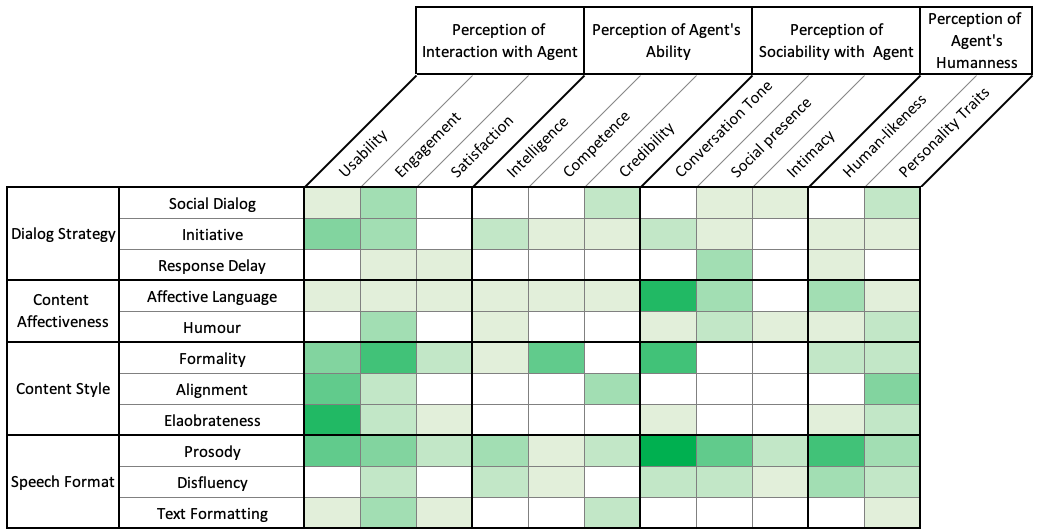
\includegraphics[width=\textwidth]{fig-heatmap-impact.png}
  \caption{Heatmap of literature for perception of conversational agents for each type of conversational architecture element.}
  \Description{This graph shows the number of papers measuring the effect of conversational architecture elements on different perception measures of conversational agents. Conversational architecture elements are categorized into content (affective language, self-disclosure, humour), format (disfluency, typo, capitalization, speech rate, response delay), and style (lexical alignment, formality, emoticons, prosody). Perceptions are categorized into perception of interaction with an agent (engagement, satisfaction, accuracy), perception of social connection with an agent (intimacy, conversation tone, social presence), and perception of agent's humanness (human-likeness, trustworthiness, personality traits).}
  \label{fig:heatmap-impact}
\end{figure*}

Figure \ref{fig:heatmap-impact}


%%%%%
\subsection{Perception of Interaction with an Agent}
%%%%%

This section discusses user's perception of their interaction with a conversational agent. \textbf{\textit{Engagement, accuracy, and satisfaction are the three variables used to evaluate how people perceive interactions with CAs}}. \textit{Engagement} measures user's attitude towards the task they are achieving through working with the agent, including how easy it is to use the system and its perceived usefulness, convenience and helpfulness for the user. Additionally, it includes the user's emotional responses to the interaction, such as annoyance, enjoyment, and irritation. \textit{Accuracy} measures whether the agent was perceived to be able to provide the correct answers in response to the user. \textit{Satisfaction} measures the whether the agent was able to fulfill user's expectations through the interaction encounter.

Out of the list of publications that were evaluated, there is a good coverage on the effect of conversational architecture elements on the perception of interaction with an agent. Out of the three factors, engagement is the most frequently used measure to assess interaction quality, followed by satisfaction. Perceived accuracy of the agent is rarely used within literature, with only a few papers measuring this perception. 

[TODO] * Associations between conversational architecture elements and perceptions
For both text and voice modalities, lexical alignment had a positive effect on engagement by decreasing the cognitive load of users. 

%%
\subsubsection{Engagement}
%%
For the elements in the language content category of conversational architecture, the use \textbf{self-disclosure} by agent had a positive effect on engagement, as the participants using the chatbot with small talk and self disclosure reported higher enjoyment after 3 weeks of daily interaction \cite{lee2020hear}\cmt{[23]}. There are mixed results on the effect of \textbf{affective language} on engagement. One study found that CAs that uses encouraging words are rated as easier to use \cite{healey2013relating}\cmt{[39]}. However, the user of words with increased lexical emotional expressiveness did not have an effect on engagement \cite{zhu2022effects}\cmt{[26]}. The use of affective language may lead to negative impacts on engagement, as a system that uses an extroverted and overly familiar words is irritating to users. On the use of \textbf{humour}, survey result did not show a significant difference in the level of enjoyment, but qualitative feedback from participants reflected that humour made the interaction more engaging and immersive \cite{ceha2021can}\cmt{[57]}.

For the elements in the language style category of conversational architecture, mimicking users' utterances through \textbf{lexical alignment} yielded positive results. Multiple studies have found that being lexically aligned to users resulted in lower perceived cognitive demand and decreased perceived workload \cite{huiyang2022improving}\cmt{[17]}\cite{linnemann2018can}\cmt{[15]}\cite{spillner2021talk}\cmt{[18]}. Interestingly, perceived lower cognitive demand did not have significant impacts on ease of use \cite{linnemann2018can}\cmt{[15]} or annoyance \cite{huiyang2022improving}\cmt{[17]}. In Spillner et al's study \cite{spillner2021talk}\cmt{[18]}, both conditions of aligning words as well as aligning words and grammatical structure to user utterances resulted in higher perceived user engagement from participants. 

For the elements in the presentation format category of conversational architecture, auditory aspects of \textbf{prosody} such as speech rate and expressive tone of voice had different impacts on engagement. In one study, users enjoyed their interaction with the CA and perceived it as easier to use, as they felt the level of agent's social behaviour is matched with their emotional states \cite{kim2020can}\cmt{[24]}. However, another study did not find any impact of emotional expressive of voice on the user engagement \cite{zhu2022effects}\cmt{[26]}. On the speech rate for CAs, a normal rate is perceived as more convenient compared to a faster rate of speech \cite{choi2020nobody}\cmt{[54]}. On the visual presentation side, the study from Westerman et al. \cite{westerman2019believe}\cmt{[9]} showed that the use of \textbf{typos} by chatbots negatively impacted the perception of working with a CA on the specific task, while the use of \textbf{capitalization} did not yield any significant impacts.

\textbf{Content: Humour}
* No overall significant difference between conventional method vs. agent using humour for enjoyment. Specifically, men enjoyed the agent's jokes more than women.  \cite{miyamoto2017improving}\cmt{[46]}.
* Motivation to continue the conversation significant increased after day 2 for the humorous agent \cite{go2021conversational}\cmt{[80]}

\textbf{Style: Language Formality}
* Users spent more time with the Shakespearean chatbot version with more non-task related user inputs. Enjoyment was measured but no report \cite{elsholz2019exploring}\cmt{[61]}
* commanding/formal wording was rated significantly more useful than the informal wording; while the informal wording was rated as significantly more annoying than the commanding/formal wording. No impact on desirability. \cite{jestin2022effects}\cmt{[81]}
* High conscientiousness (formal) and high extroversion (casual) chatbot personality have higher user engagement. \cite{moilanen2022measuring}\cmt{[82]}
* Analysis of ease of use reveals that there are no significant main effects for platform questionnaire vs. chatbot, and conversational style formal vs. casual.\cite{kim2019comparing}\cmt{[89]}

\textbf{Social talk / elaborate}
* Not significant importance between introvert and extrovert agents. But the machine-like speaking agent is rated lower. \cite{roy2021users}\cmt{[71]}
* usefulness depended on the task \cite{haas2022keep}\cmt{[78]}
* High extroversion chatbot personality have the higher user engagement \cite{moilanen2022measuring}\cmt{[82]}

\textbf{Disfluency}
* Using moderately repetitive utterances resulted in higher desire to continue the dialogue with the agent. \cite{yang2021effect}\cmt{[72]}
* Interjections did not have any impacts of cognitive workload \cite{ceha2022expressive}\cmt{[77]}

\textbf{Proactive}
* Different framing has impacts on the perceived disruptiveness of the agent. \cite{xiao2021let}\cmt{[73]}

\textbf{Prosody}
* No impact on annoying, undesirable, useful \cite{jestin2022effects}\cmt{[81]}
* Dialog-style conversation using prosodic cues is rated as less easy to understand than the reading-style \cite{misu2011toward}\cmt{[83]}

\textbf{Combined}
* (Extraverted: emoticons, self-disclosure, talkative, affective language / Introverted: formal style, less talkative) all personalities have similar usability ratings. Also, users have greater desire to interact with the extraverted chatbot \cite{volkel2022user}\cmt{[75]}
* (Politeness: affective language + elaborateness of speech) no impact on usability \cite{hu2022polite}\cmt{[76]}


%%
\subsubsection{Accuracy}
%%
There are only a few studies that measured the perception of accuracy of conversational agents for an interaction. A couple of studies reported the effect of the use of language style of \textbf{lexical alignment}. One study of a text-based CA resulted in higher perceived response accuracy \cite{huiyang2022improving}\cmt{[17]}, while the other study with voice-based CA did not find any significant differences \cite{linnemann2018can}\cmt{[15]}. Dubiel et al.'s study \cite{dubiel2020persuasive}\cmt{[60]} on \textbf{prosody} did not find any significant differences on the rating for accuracy across agents with different speech rates and pitch.

\textbf{Social talk}
* Introverted agent is more efficient. \cite{roy2021users}\cmt{[71]}
* Efficiency depended on the task \cite{haas2022keep}\cmt{[78]}

\textbf{Language Formality}
* commanding/formal wording was rated significantly more effective than informal wording \cite{jestin2022effects}\cmt{[81]}

\textbf{Prosody}
* No impact on effectiveness \cite{jestin2022effects}\cmt{[81]}

\textbf{Repair}
* One reason for choosing repair strategy preference is efficiency and efficacy. \cite{ashktorab2019resilient}\cmt{[88]}

%%
\subsubsection{Satisfaction}
%%
Several research have investigated into how the usage of \textbf{affective language} impacts the satisfaction people feel when interacting with a CA. Compared to a text-based chatbot with a static and neutral response, users reported higher service encounter satisfaction conversing with a chatbot that responded with dynamic, sentiment-adaptive responses \cite{diederich2019emulating}\cmt{[25]}. However, the same effect is not observed for a voice-based CA as Yang et al. did not find any difference in user satisfaction rating between the emotional-expressing agent vs. non-emotional expressing agent \cite{yang2017perceived}\cmt{[44]}. On the language style used by CAs, both \textbf{disfluency} \cite{pfeifer2009should}\cmt{[12]} and \textbf{emoticons} \cite{wilhelm2022keep}\cmt{[28]} did not have any significant effects on user satisfaction.

Studies have found that presentation formats have significant effects on user satisfaction. In Choi et al's study \cite{choi2020nobody}\cmt{[54]} on the speech rate aspect o f\textbf{prosody} for a voice-based agent, they found that user satisfaction is higher for the default rate compared to using a faster rate. User feedback reflected that the faster rate was mechanical and harder to understand. For text-based chatbots, the addition of \textbf{response delay} increased the perception of overall user satisfaction, as the timing is similar to human-human communications and felt right \cite{gnewuch2018faster}\cmt{[19]}. 

\textbf{Style: Language Formality}
* Modern language had higher usability score compared to Shakespearean language \cite{elsholz2019exploring}\cmt{[61]}
* There is no significant effect on customer satisfaction of the CA between low-status and high-status languages. \cite{habler2019effects}\cmt{[63]}

\textbf{Format: Prosody}
* There is no significant effect on customer satisfaction of the CA between male-gendered and female-gendered voices. \cite{habler2019effects}\cmt{[63]}

\textbf{Social talk}
* Not significant importance between introvert and extrovert agents. But the machine-like speaking agent is rated lower. \cite{roy2021users}\cmt{[71]}

\textbf{Combined}
* (Politeness: affective language + elaborateness of speech) no impact on user satisfaction \cite{hu2022polite}\cmt{[76]}

%%%%%
\subsection{Perception of Agent's Ability}
%%%%%

This section discusses how user perceives the agent's ability in conditions with different conversational architecture elements. It is aiming at measuring the differences in the perception with similar system's capabilities. Out of the two variables used to evaluate this perception, \textit{Intelligence} measures whether the agent is knowledgeable, sensible, and is seem as overall intelligent. \textit{Competence} on the other hand measures the overall perception on how well the agent is handling the conversation. Out of the list of publications that were evaluated, there are only a few papers that measured the perceived ability of an agent.

\textit{To be incorporated}

\textbf{Repair}
* perceived quality of the interaction is muhc higher in repair condition when the agent made a mistake; rating is lower if no mistake was present. \cite{cuadra2021my}\cmt{[67]}

%%
\subsubsection{Intelligence}
%%

On analyzing the impact of different language styles on the perception of intelligence, a couple of papers studied the effect of including \textbf{disfluencies} into agent's speech. One paper found that there is no significant impact on how knowledgeable the agent is perceived as \cite{pfeifer2009should}\cmt{[12]}. Another study showed that using fillers like "um" and "uh" decreased the agent's perceived intelligence overall \cite{jeong2019exploring}\cmt{[10]}. Upon further analysis, the authors noticed a difference between task vs. social conversations, as users perceive the intelligence to be lower in task-oriented situations, but the perception of intelligence is slightly increased in social-oriented situations. The use of \textbf{lexical alignment} did not seem to impact user's perception of an agent's intelligence, as there is no significant difference reported in the agent's domain knowledge between the aligned vs. non-aligned conditions.

On the impact of presentation format, Dubiel et al's study on \textbf{prosody} using different speech rates and pitches did not yield any significant differences on the agent rating for knowledgeable.

\textbf{Prosody}
* VA using kin's voice is rated as more intelligent. \cite{chan2021kinvoices}\cmt{[74]}

\textbf{Repair}
* One reason for choosing repair strategy preference is perceived intelligence and capability. \cite{ashktorab2019resilient}\cmt{[88]}

%%
\subsubsection{Competence}
%%

There are only a couple of papers that discussed the impact of conversational architecture elements on the perception of competence. For \textbf{affective language} in the language style content category, participants rated the agent higher in competence when it has higher patiency and expressed its feelings to users. In Cox et al's study on \textbf{formality}, the authors did not find a significant difference in competence between using casual vs. formal conversational styles.

\textbf{Style: Language Formality}
*  Low-status language resulted in higher achieved performance ratings \cite{habler2019effects}\cmt{[63]}

\textbf{Format: Prosody}
* There is no significant effect on perceived performance of the CA between male-gendered and female-gendered voices. \cite{habler2019effects}\cmt{[63]}
* For expertise, multilingual students rated higher the non-native English-speaking virtual human. \cite{feijoo2021effects}\cmt{[70]}

\textbf{Format: Proactivity}
* Certain proactive styles like notification strategy (conservatively proactive, letting participants know that the agent has found a solution) was evaluated as significantly higher perceived competence compared to the non-strategy. \cite{kraus2020effects}\cmt{[64]}



%%%%%
\subsection{Perception of Social Connection with an Agent}
%%%%%

This section discusses user's perception of their social connection with a conversational agent. Social presence, conversation tone, and intimacy are the three variable used to evaluate this perception. \textit{Social presence} measures user's perceived social distance with an agent, such as social presence, connectedness, and psychological distance. \textit{Conversation tone} measures user perceptions on the way an agent is speaking to them, such as appropriateness of tone, empathetic, or emotionally expressive. \textit{Intimacy} measures the quality of relationship users have with CAs, such as intimacy, social attraction, or similarity with each other.

Out of the list of publications that were evaluated, there is overall consensus that the use of affective language positive affects the perception of social connection with an agent. Conversational architecture elements related to the format of the conversation, like adding response delays, or changing the pitch of speech are commonly investigated for perception of social connection with an agent. There are only a few papers exploring the effect of language styles on the perceived social connection with an agent. 

%%
\subsubsection{Social Presence}
%%
For conversational architecture elements related to language content, studies have shown the use of \textbf{affective language} increased the perception of social presence of an agent. In Diederich et al's study, participants conversing with a text-based agent using dynamic, sentiment-adaptive responses reported a higher social presence compared to a CA that provides static, neutral responses \cite{diederich2019emulating}\cmt{[25]}. In another study, participants felt closer to the agent psychologically when the CA expressed its feelings \cite{lee2019s}\cmt{[55]}. On the use of \textbf{humour}, Lee et al. did not find any significant difference in social presence between the humourous and non-humourous agent \cite{lee2019s}\cmt{[55]}.

For text-based conversational agents, including a \textbf{response delay} increased users' perception of social presence of the agent, with participants feeling a sense of human contact and sociability with the agent \cite{kim2020can}\cmt{[24]}. Westerman et al. \cite{westerman2019believe}\cmt{[9]} studied the presence of typos and capitalized words in a text-based agent's responses. They found the inclusion of \textbf{typos} negatively impacted the social distance and connection with an agent, while \textbf{capitalization} did not have any significant effects. On the effect \textbf{prosody} on a voice-based agent, using an affective tone of voice resulted in perceived higher social connectedness with the agent \cite{kim2020can}\cmt{[24]}.

\textbf{Content: Affective Language (Voice)}
* Model aiming to elicit position emotions from users received higher emotional connection \cite{lubis2019positive}\cmt{[43]}

\textbf{Format: Response Delay}
* Delayed response is associated with higher social presence \cite{gnewuch2022opposing}\cmt{[20]}

\textbf{Content: Affective language and Style: Disfluency}
* Rated higher that agent listened openly to participants' emotions, as that agent can feel waht the user is feeling. \cite{hu2021enhancing}\cmt{[56]}
* social condition didn't have an impact on social presence \cite{lubold2016effects}\cmt{[86]}

\textbf{Prosody}
* VA using kin's voice is rated as more socially present and closer psychological connection with user. \cite{chan2021kinvoices}\cmt{[74]}
* voice plus social condition has higher social presence than the social condition \cite{lubold2016effects}\cmt{[86]}

\textbf{Humour}
* Familiarity with the agent is rated higher at the end of the study (day 7) compared to non-humorous agent \cite{go2021conversational}\cmt{[80]}

\textbf{Laughter}
* Laughter had no impact on social presence of an agent \cite{niewiadomski2013laugh}\cmt{[85]}

%%
\subsubsection{Conversation Tone}
%%

The use of \textbf{affective language} has a significant affect on the perception of the conversation tone by the agent. Multiple studies have found that agents conversing with more affective words are seen as more emotionally expressive and empathetic \cite{daher2020empathic}\cmt{[58]}\cite{diederich2019emulating}\cmt{[25]}\cite{yang2017perceived}\cmt{[44]}\cite{zhu2022effects}\cmt{[26]}. This effect has been observed across modalities in both text-based as well as voice-based conversational agents.

On the style of language used by the agent, \textbf{formality} did not seem to impact the conversation tone of agent as Cox et al. \cite{cox2022does}\cmt{[27]} did not find any significant difference between casual and formal conversational styles for appropriateness of tone. The speech format of \textbf{prosody} seem to have an impact on the conversation tone, as a CA speaking with a lower pitch and slower speech rate is rated as more persuasive compared to other voice settings \cite{dubiel2020persuasive}\cmt{[60]}. However, there was no significant difference in how powerful or bold the agent's tone was perceived across various prosody settings.

\textbf{Content: Affective language and Style: Disfluency}
Respond with empathy to the user. \cite{hu2021enhancing}\cmt{[56]}

\textbf{Disfluency}
* Using moderately repetitive utterances resulted in higher perceived empathy. \cite{yang2021effect}\cmt{[72]}

\textbf{Language Formality}
* commanding/formal wording was rated significantly more appropriate and assertive than informal wording \cite{jestin2022effects}\cmt{[81]}

\textbf{Prosody}
* No impact on appropriate and assertive \cite{jestin2022effects}\cmt{[81]}
* Dialog-style conversation using prosodic cues is rated as more appropriate than the reading-style \cite{misu2011toward}\cmt{[83]}

%%
\subsubsection{Intimacy}
%%
On the use of language content, a conversational agent that included \textbf{self-disclosure} when conversing with participants resulted in higher level of intimacy over time than CAs that did not self disclose \cite{lee2020hear}\cmt{[23]}. On the other hand, using the style of \textbf{lexical alignment} by using the words that were already used by the participant did not result in higher quality of relationship with the agent \cite{linnemann2018can}\cmt{[15]}.

There are several studies investigating the effect of conversational format on intimacy with a CA. Specifically on voice \textbf{prosody}, using an affective tone of voice increased the perceived intimacy and similarity with an agent \cite{kim2020can}\cmt{[24]}. Comparing voice agents with different \textbf{speech rates}, users rated the default rate as more intimate than a faster rate of speech \cite{choi2020nobody}\cmt{[54]}, noting that the default rate is more human-like and natural. Westerman et al's study on different text formats of conversation \cite{westerman2019believe}\cmt{[9]} showed that \textbf{typos} negatively impacted the perceived social attraction of the agent, while \textbf{capitalization} did not have any impacts.

\textbf{Disfluency}
* Interjections did not have any impacts of quality of relationship, but it did result in higher emotional rapport. \cite{ceha2022expressive}\cmt{[77]}

\textbf{Affective Language}
* social condition didn't have an impact on social presence \cite{lubold2016effects}\cmt{[86]}

\textbf{Prosody}
* voice and social condition didn't have an impact on social presence \cite{lubold2016effects}\cmt{[86]}

%%%%%
\subsection{Perception of Agent's Humanness}
%%%%%

This section discusses user's perception of the agent's humanness aspects. Human-likeness, personality traits, and trustworthiness are the three variable used to evaluate this perception. \textit{Human-likeness} measures the agent's similarity to humans as well assessed naturalness of interaction. \textit{Personality traits} measures perceptions of the agent's characteristics such as likeability, warmth, and friendliness. \textit{Trustworthiness} measures if users feel they can trust an agent, and whether the agent is perceived of being truthful.

Out of the list of publications that were evaluated, many papers exploring the impact of language content as well as language style have measurements related to the perception of an agent's humanness. There seems to be fewer studies looking into the effect of conversation format on the perception of agent's humanness, as our reivew only found two studies related to voice prosody. Out of reviewed conversational architecture elements, one consistent finding is that the style of being lexically aligned with user's utterance did not have any impact on the perception of agent's humanness.

%%
\subsubsection{Human-likeness}
%%

On the use of \textbf{affective language}, one study found that CAs with dynamic, sentiment-adaptive responses is perceived as more human than a CA that provides static, neutral responses \cite{diederich2019emulating}\cmt{[25]}. Another study using more emotional expressive words in conversation did not find any significant impact on the perceived human-likeness of an agent \cite{zhu2022effects}\cmt{[26]}.

Different language styles have different impacts on user perceptions. On language \textbf{formality}, agents using normal style was rated as more human-like compared to formal styles of conversation \cite{ouchi2019should}\cmt{[59]}. \textbf{Disfluencies} did not seem to have a significant impact on the perceived humanness or naturalness of an agent \cite{jeong2019exploring}\cmt{[10]}\cite{pfeifer2009should}\cmt{[12]}. However, one study noticed a non-significant but positive trend in user's evaluation of the agent using fillers as being more human-like \cite{jeong2019exploring}\cmt{[10]}.

On the impact of different conversation formats, Zhu et al. did not find a significant effect of \textbf{prosody} on the perception of humanness between agent using expressive vs. non-expressive voices. For text-based CAs, the use of \textbf{typos} made the agent seem less human, while the use of \textit{capitalization} did not have any impacts on the perception of humanness \cite{westerman2019believe}\cmt{[9]}. Lastly, adding a \textbf{response delay} to a CA has a significant positive effect in the perceived humanness of the agent \cite{gnewuch2018faster}\cmt{[19]}. 


\textbf{Style: Disfluency}
* (Voice) No significant difference in naturalness rating for About Myself text, but showed that naturalness is higher for fluent system compared to disfluent speech \cite{wester2015artificial}\cmt{[14]}.

\textbf{Prosody}
* VA using kin's voice is rated as more human-like. \cite{chan2021kinvoices}\cmt{[74]}
* Dialog-style conversation using prosodic cues is rated as less human-like than the reading-style \cite{misu2011toward}\cmt{[83]}

\textbf{Social talk / Elaborateness}
* Naturalness depends on the task \cite{haas2022keep}\cmt{[78]}

\textbf{Language Formality}
* No impact on artificial or humanlike perceptions \cite{jestin2022effects}\cmt{[81]}

\textbf{Prosody}
* Matthew voice is rated as least artificial  \cite{jestin2022effects}\cmt{[81]}

\textbf{Laughter}
* Laughter was not rated as natural in an agent \cite{niewiadomski2013laugh}\cmt{[85]}

\textbf{Combined}
* (Politeness: affective language + elaborateness of speech) no impact on likability, but positive politeness interactions are rated as more polite \cite{hu2022polite}\cmt{[76]}

\textbf{Repair}
* One reason for choosing repair strategy preference is naturalness. \cite{ashktorab2019resilient}\cmt{[88]}


%%
\subsubsection{Personality Traits}
%%

There are significant difference found in the effect of language content on the perception of agent's personality traits. Conversational agents using emotionally expressive words are rated as more likable \cite{zhu2022effects}\cmt{[26]} and warm \cite{lee2019s}\cmt{[55]}. In Healey et al's study \cite{healey2013relating}\cmt{[39]}, there is a significant difference in the variances of the responses for friendliness of the agent between the agent using encouraging words compared to neutral utterances. As with the use of \textbf{humour}, participants rated the humorous agent as having a sense of humor, but it was not rated as more likable \cite{ceha2021can}\cmt{[57]}.

On the impact of language style, various studies on \textbf{lexical alignment} showed that there is no significant impact on the perception of the personality traits related to likability \cite{huiyang2022improving}\cmt{[17]}\cite{linnemann2018can}\cmt{[15]}, friendliness \cite{spillner2021talk}\cmt{[18]}, or politeness \cite{spillner2021talk}\cmt{[18]}. Studies on the \textbf{formality} of language has demonstrated that casual conversational style is perceived as warmer than formal style \cite{cox2022does}\cmt{[27]}. Also agents using a normal style as compared to a formal style is perceived as more friendly, fun, and kind \cite{ouchi2019should}\cmt{[59]}. As for the use of \textbf{disfluency}, there was no statistical significance found in the perceived likability rating \cite{jeong2019exploring}\cmt{[10]}\cite{pfeifer2009should}\cmt{[12]}. Jeong et al. \cite{jeong2019exploring} found a significant interaction effect between disfluency (using fillers) and the context of the conversation (task vs. social), as users considered agents using fillers as entertaining and fun in social conversations, but inappropriate in task oriented situations.

In the list of reviewed papers, there was only one study measuring the perceived trustworthiness of an agent based on different conversational format of \textbf{prosody}. Dubiel et al. found that an agent using slower speech rate is perceived as more trustworthy as compared to other voice prosody settings \cite{dubiel2020persuasive}\cmt{[60]}.

\textit{To be incorporated}

\textbf{Content: Humour}
* An agent that uses humourous content is assessed to be more funny \cite{khooshabeh2011does}\cmt{[37]}.

\textbf{Style: Disfluency}
* (Voice) Both About Myself and Speed Dating ratings has shown system scored significantly differently on the Big-5 personality traits. Disfluency makes the voice sound more neurotic, less open, less extrovert and less conscientious \cite{wester2015artificial}\cmt{[14]}.

\textbf{Format: Prosody}
* Low voice pitch rated not as friendly as the other ones. No impact on other traits like assertive and politeness. \cite{tolmeijer2021female}\cmt{[62]}
* VA using kin's voice is rated as more likable. \cite{chan2021kinvoices}\cmt{[74]}
* No impact on entertaining or friendly  \cite{jestin2022effects}\cmt{[81]}

\textbf{Repair}
* When VA corrected in the condition it didn't make a mistake, it is seen as anxious. Otherwise it is perceived as calm and emotionally stable. \cite{cuadra2021my}\cmt{[67]}
* One reason for choosing repair strategy preference is politeness. \cite{ashktorab2019resilient}\cmt{[88]}

\textbf{Social talk}
* Using more social talk is positive correlated with extroversion. \cite{volkel2021manipulating}\cmt{[68]}
* Not significant importance between introvert and extrovert agents. \cite{roy2021users}\cmt{[71]}
* Likability depends on the task \cite{haas2022keep}\cmt{[78]}

\textbf{Language Formality}
* Informal wording was rated as strongly more entertaining and friendly than the commanding/formal wording. \cite{jestin2022effects}\cmt{[81]}

\textbf{Agreeableness}
* Being highly confrontational (less agreeable) is rated as less conscientious \cite{volkel2021manipulating}\cmt{[68]}
* Designing for more agreeable resulted in personality rated as more agreeable \cite{volkel2021examining}\cmt{[69]}

\textbf{Combined}
* (Extraverted: emoticons, self-disclosure, talkative, affective language / Introverted: formal style, less talkative) extraverted personality rated as more extraverted \cite{volkel2022user}\cmt{[75]}

%%
\subsubsection{Trustworthiness}
%%

For the use of language content, agents using more \textbf{affective language} is seen as less trustworthy, as users felt it was being overly familiar \cite{andrews2012system}\cmt{[38]}. On the other hand, users conversing with agents that used \textbf{self-disclosure} content reported more trust towards the agent compared to the non disclosure group \cite{lee2020hear}\cmt{[23]}.

None of the studies included in this review has found any significant impact of language style, \textbf{lexical alignment} \cite{hoegen2019end}\cmt{[31]}\cite{huiyang2022improving}\cmt{[17]}\cite{linnemann2018can}\cmt{[15]}, \textbf{disfluency} \cite{pfeifer2009should}\cmt{[12]}, and \textbf{emoticons} \cite{wilhelm2022keep}\cmt{[28]} on the perceived trustworthiness of CAs. Similarly for conversational format, there is not significant difference on the rating for truthfulness of the agent across different voice \textbf{prosody} settings \cite{dubiel2020persuasive}\cmt{[60]}.

\textbf{Format: Prosody}
* No significant difference in trust ratings across different voice prosody settings with differences in pitch. \cite{tolmeijer2021female}\cmt{[62]}
* No impact on trustworthiness  \cite{jestin2022effects}\cmt{[81]}

\textbf{Format: Proactivity}
* Overall trust in the system did not differ significantly. The intervention style is less trusted than conservative strategies - too obstructive and imposing. Proactive should be subtle  \cite{kraus2020effects}\cmt{[64]}

\textbf{Language Formality}
* No impact on trustworthiness \cite{jestin2022effects}\cmt{[81]}


%-------------
\section{Discussions}

%Research challenges and opportunities

%Ethical considerations

%Limitations and future work

\subsection{RQ1 - synthesis of conversation architecture elements}

Sometimes a study is covering multiple conversational element cues, hard to break it out. For example, extroverted personality used in \cite{volkel2022user}\cmt{[75]} has emoticons, affective language, talkative, and self-disclosure. Need to break it down.

Also, breaking down "personalities" to its core components.


\subsection{RQ2 - synthesis of perceptions}

\subsubsection{Inconsistencies in Perception Measures}

A major roadblock in synthesizing the findings from existing academic research is the diversity and inconsistency of measurements towards the anthropomorphized perception of agents. It is difficult to assess whether perception measures should be compared with each other. Also, some measures combined anthropomorphized perceptions into a composite score, which makes it impossible to separate the perceptions into more granular details.

Based on the literature reviewed in this paper, we noticed that similar perception concepts were \textbf{measured in different ways} through different surveys. For example, there are several approaches to measure the perceived \textit{human-likeness} of an agent. A commonly used survey is adapted from the Godspeed questionnaire \cite{bartneck2009measurement}, which measures human-likeness based on user's impression of the agent as fake / natural, machinelike / humanlike, unconscious / conscious, and artificial / lifelike (used by \cite{hoegen2019end}\cmt{[31]}, \cite{jeong2019exploring}\cmt{[10]} and \cite{ouchi2019should}\cmt{[59]}). Another way to measure human-likeness is adapted from Holtgraves et al.'s \cite{holtgraves2007perceiving} questionnaire, which asks users to assess the agent's perceived human-likeness, skillfulness, thoughtfulness, politeness, responsiveness and engagement (used by \cite{diederich2019emulating}\cmt{[25]} and  \cite{gnewuch2018faster}\cmt{[19]}). One study \cite{westerman2019believe}\cmt{[9]} used the Ascend of Man pictorial scale \cite{kteily2015ascent} as the measure of perceived human-likeness. It is unclear whether these different measures of perceived human-likeness are similar enough to be compared with each other.

 In addition to different methods used to measure for the same perception, our detailed analysis revealed that the measures using the same label may have \textbf{drastically different meanings}. In Diedrech et al.'s study \cite{diederich2019emulating}\cmt{[25]}, \textit{empathy} measure is adapted from \cite{yan2013role} assessing whether the CA gives users individual or personal attention. In Daher et al.'s study \cite{daher2020empathic}\cmt{[58]}, they also measure the perception of empathy, but it is using the RoPE Scale \cite{charrier2019rope} with questions like "the robot cares about my feelings" or "the robot comforts me when I am upset." These two different measures of empathy seem to have different underlying meanings, one assessing the personalization aspect of CAs, while the other is assessing the emotional aspect of CAs. Another example is the measurement of \textit{trustworthiness}, with some constructs measuring the level of sensitive information user's are willing to share \cite{dinev2006privacy}, and some measuring the honesty and truthfulness of an agent \cite{lee2017enhancing}. 

Lastly, there are \textbf{composite measures} of anthropomorphized perception across different categories, making it difficult to break down perceptions into granular details for analysis. One such example is Ma et al's study \cite{ma2022ask}\cmt{[29]} on different approaches for CAs to reply to users' uncertain queries. UX score is used to measure the perception of an agent, which asks whether the user thinks the CA's response is pleasing / trustworthy / natural / acceptable / shorten the distance between CA and user. While the study has found significant impact of the use of formal language on UX score, it is not possible to breakdown the measure into perceptions of interaction (pleasing, acceptable), social connection (shorten the distance between CA and user), and humanness (natural, trustworthy). Similar for Hoegen et al.'s study \cite{hoegen2019end}\cmt{[31]} on the impact of conversational style matching, it is not possible to separate the overall interaction score into different perceptions as the composite measure contains questions measuring different categories of perceptions like interaction (engaging) and humanness (trust, likable).

In recent years there has been some effort towards unifying the evaluation of conversational agents, such as the work by Finch et al. \cite{finch2020towards} presenting a comprehensive analysis of current evaluation protocols. More work is needed to categorize and consolidate perception measures to make them consistent and comparable across various studies. 

%For discussions on mental well beings, agent using emojis is rated higher for attitude (emotional connection) . However, for agent with discussing physical well being, agent using emojis is rated as lower for attitude. 
%Attitude has emotional connection, coherent - coherent is an ability perception, vs. emotional connection is a social connection perception. \cite{fadhil2018effect}\cmt{[52]}

\subsubsection{Relationship between perceptions}

Response delay: social presence has a significant effect on intention to use. 
\cite{gnewuch2022opposing}\cmt{[20]}

Perceived intelligence positively associated with perceived usefulness, perceived ease of use, initial trust, and perceived anthropomorphism. Perceived anthropomorphism is associated with perceived enjoyment, and intention to adopt. Perceived usefulness and perceived enjoyment impacts intention to adopt. \cite{moussawi2021perceptions}\cmt{[36]}

The size of the effect for language we observed is clearly higher than the size of the effect for voice. \cite{habler2019effects}\cmt{[63]}

VA self-repair can backfire if time or accuracy is of the essence. (repair and accuracy) \cite{cuadra2021my}\cmt{[67]}


\subsection{RQ3 - relationship between conversation architecture elements and perceptions}

\subsubsection{Other Influencing Factors}

While the discussion in the Framework section above focuses on the overall effect of conversational architecture elements on anthropomorphized perceptions,  there are other nuanced influencing factors that impact user perceptions of agents. 

Depending on the \textbf{type of conversation} user is having with agents, it may lead to differences in perceptions for similar conversational architecture elements. Cox et al. \cite{cox2022does}\cmt{[27]} found that the perceived competence and appropriateness of tone of different language formality styles depend on the sensitivity of information discussed in the conversation. In this particular study, a formal language style is preferred in medical history discussions as it is matching to the expectation of users, but there is no difference in perception between formal and casual styles when discussing income level and credit scores. In Jeong et al's study \cite{jeong2019exploring}\cmt{[10]}, users found the agent using fillers less intelligent and likable in a task-oriented conversation, but found the same agent using fillers as slight more intelligent and likable in a social-oriented conversation. Another factor that could impact perceptions is the \textbf{anonymity} of conversation. Based on user feedback, Lee et al. \cite{lee2020hear}\cmt{[23]} found that the anonymity of a conversational agent is a driving factor encouraging people to self disclose without having to worried about judgements from the CA. The perception of the agent may be different if the user's identity is not anonymous.

Other than the type of conversation, \textbf{user's characteristics} can also be influencing factors on their perception of agents. For example, the effect of matching user's conversational style on perception of agents depend on user's own conversational style, as participants with high consideration conversational style rated the lexically aligned agent as more trustworthy \cite{hoegen2019end}\cmt{[31]}. In the study by Cox et al. \cite{cox2022does}\cmt{[27]}, participants with lower levels of privacy concerns as well as those who believe in robotic intelligence found the chatbot more enjoyable, warm, competent and appropriate. Similarly, participants with positive attitudes towards computers were significantly more likely to indicate that the usage of fillers by agents was a positive aspect of the conversation, compared to participants with neutral attitudes towards computers \cite{pfeifer2009should}\cmt{[12]}. Lastly, user's prior experience with conversational agents could impact perception of agents. Experienced users perceived the agent with a response delay as lower in social presence compared to the one without delay, as it is seen as inefficient to wait for the CA to respond. However, novice users perceived higher social presence conversing with the CAs using response delays as it is more similar to conversations with human partners \cite{gnewuch2018faster}\cmt{[19]}.

* Format: Response delay - Novice users perceived the agent as more socially present, but experienced users had a negative effect \cite{gnewuch2022opposing}\cmt{[20]}
* Content: Humour - no overall significant difference between conventional method vs. agent using humour for enjoyment. Specifically, men enjoyed the agent's jokes more than women.  \cite{miyamoto2017improving}\cmt{[46]}.
* Format: Proactivity - significant interaction between proactive dialogue strategies and task difficulty for perceived competence and perceived reliability. For easier tasks, system help is not really required. \cite{kraus2020effects}\cmt{[64]}
* Preference for the level of social talk depended on the task, even within the same transactional context, as users preferred high level for playing a song, but low level for writing a text. \cite{volkel2021manipulating}\cmt{[68]}
* Correlation between user's personality of agreeableness vs. preference for agreeable level of chatbot \cite{volkel2021examining}\cmt{[69]}
* For expertise, multilingual students rated higher the non-native English-speaking virtual human. \cite{feijoo2021effects}\cmt{[70]}
* Participants felt irritated when humorous statements were made when they talked about experiencing sadness \cite{go2021conversational}\cmt{[80]}

%\subsubsection{Study Design}

%\textbf{Interview vs experiment}
%* Humour - what's said vs. study results

%\textbf{Observer study vs. interaction study}
%* In observer study, participants attributed higher integrity (trustworthiness), response accuracy and likeability to the agent with lexical alignment, but this effect was not observed in the interaction study. Also, interaction study had lower cognitive demand but no effect in the observer study. \cite{linnemann2018can}\cmt{[15]}
%* \cite{zhu2022effects}\cmt{[26]}
%* \cite{cox2022does}\cmt{[27]}


\subsubsection{Modality}

TBD 
Did not separate - because similar 
Affective language - may be a difference? significant for text, but not as much for voice?


\subsubsection{Gaps}

Combined effects
* integrated mental model \cite{knijnenburg2016inferring}\cmt{[34]}
* Anthropomorphized chatbot (text) using affective language (emotional expressions), self-referencing, emoticons, response delays. Resulted in higher perceived anthropomorphism, which in result led to lower negative word of mouth and loss of trust. anthropomorphic design is beneficial not only to initial trust but also to the ongoing trust relationship \cite{seeger2021chatbots}\cmt{[35]}

Lack of investigations - name a few areas

%\subsubsection{Human-human vs. Human-machine}

%* Impact of lexical alignment on people's perceived annoyance and likability differed in HHI (higher) and HCI (no impact). \cite{huiyang2022improving}\cmt{[17]}.

\subsubsection{Ethical Considerations}

Self-disclosure encourage higher trust and intimacy, to disclose sensitive information. Who have access to this data? need to be aware of privacy / data sharing practices. \cite{lee2020hear}\cmt{[23]}

Evidence for the influence of voice gender and pitch on stereotypical trait attribution. Active trait attribution is missing as most participants attributes to the negative side of traits for CAs. \cite{tolmeijer2021female}\cmt{[62]}

The social and emotional benefits of self-repair in interaction need to be balanced against the creepiness of the monitoring and modelling needed to make self-repair possible. \cite{cuadra2021my}\cmt{[67]}

\section{Conclusions}

TBD


%%
%% The acknowledgments section is defined using the "acks" environment
%% (and NOT an unnumbered section). This ensures the proper
%% identification of the section in the article metadata, and the
%% consistent spelling of the heading.
\begin{acks}
To Robert, for the bagels and explaining CMYK and color spaces.
\end{acks}

%%
%% The next two lines define the bibliography style to be used, and
%% the bibliography file.
\bibliographystyle{ACM-Reference-Format}
\bibliography{references}

%%
%% If your work has an appendix, this is the place to put it.
\appendix

\end{document}
\endinput
%%
%% End of file `paper.tex'.
